%\documentclass[10pt,notes]{beamer}       % print frame + notes
%\documentclass[10pt, notes=only]{beamer}   % only notes
\documentclass[11pt]{beamer}              % only frames

%%%%%% IF YOU WOULD LIKE TO CREATE LECTURE NOTES COMMENT OUT THE FOlLOWING TWO LINES
%\usepackage{pgfpages}
%\setbeameroption{show notes on second screen=bottom} % Both

\usepackage{graphicx}
\DeclareGraphicsExtensions{.pdf,.png,.jpg}
\usepackage{color}
\usetheme{winslab}
\usepackage[utf8]{inputenc}
\usepackage[english]{babel}
\usepackage{amsmath}
\usepackage{amsfonts}
\usepackage{amssymb}




\usepackage{algorithm2e,algorithmicx,algpseudocode}
\algnewcommand\Input{\item[\textbf{Input:}]}%
\algnewcommand\Output{\item[\textbf{Output:}]}%
\newcommand\tab[1][1cm]{\hspace*{#1}}

\algnewcommand{\Implement}[2]{\item[\textbf{Implements:}] #1 \textbf{Instance}: #2}%
\algnewcommand{\Use}[2]{\item[\textbf{Uses:}] #1 \textbf{Instance}: #2}%
\algnewcommand{\Trigger}[1]{\Statex{\textbf{Trigger:} (#1)}}%
\algnewcommand{\Events}[1]{\item[\textbf{Events:}] #1}%
\algnewcommand{\Need}[1]{\item[\textbf{Needs:}] #1}%
\algnewcommand{\Event}[2]{\Statex \item[\textbf{On#1:}](#2) \textbf{do}}%
\algnewcommand{\Trig}[3]{\State \textbf{Trigger}  #1.#2 (#3) }%
\def\true{\textbf{T}}
\def\false{\textbf{F}}


\author[Ahmet Kürşad Şaşmaz]{Ahmet Kürşad Şaşmaz\\\href{mailto:kursad.sasmaz@metu.edu.tr}{kursad.sasmaz@metu.edu.tr}}
%\author[J.\,Doe \& J.\,Doe]
%{%
%  \texorpdfstring{
%    \begin{columns}%[onlytextwidth]
%      \column{.45\linewidth}
%      \centering
%      John Doe\\
%      \href{mailto:john@example.com}{john@example.com}
%      \column{.45\linewidth}
%      \centering
%      Jane Doe\\
%      \href{mailto:jane.doe@example.com}{jane.doe@example.com}
%    \end{columns}
%  }
%  {John Doe \& Jane Doe}
%}

\title[Raymond's Algorithm]{Raymond's Algorithm}
\subtitle[Mutual Exclusion in Distributed Systems]{Mutual Exclusion in Distributed Systems}
%\date{} 

\begin{document}

\begin{frame}[plain]
\titlepage
\note{In this talk, I will present .... Please answer the following questions:
\begin{enumerate}
\item Why are you giving presentation?
\item What is your desired outcome?
\item What does the audience already know  about your topic?
\item What are their interests?
\item What are key points?
\end{enumerate}
}
\end{frame}

\begin{frame}[label=toc]
    \frametitle{Outline of the Presentation}
    \tableofcontents[subsubsectionstyle=hide]
\note{ The possible outline of a talk can be as follows.
\begin{enumerate}
\item Outline 
\item Problem and background
\item Design and methods
\item Major findings
\item Conclusion and recommendations 
\end{enumerate} Please select meaningful section headings that represent the content rather than generic terms such as ``the problem''. Employ top-down structure: from general to more specific.
}
\end{frame}
%
%\part{This the First Part of the Presentation}
%\begin{frame}
%        \partpage
%\end{frame}
%
\section{The Problem}
%\begin{frame}
%        \sectionpage
%\end{frame}

\begin{frame}{The Problem}
\framesubtitle{Selecting owner of a resource without any conflict}
\begin{block}{Mutual Exclusion in Distributed Systems} 
Mutual exclusion in distributed systems refers to the challenge of properly accessing a shared resource at any given time by different concurrent processes on different machines. The motivation is ensuring that only one process holds the resource and this resource is orderly accessed for all participants in the system by using coordination and synchronization systems.
\end{block}
\note{}
\end{frame}

\section{Our Motivation}
\begin{frame}
\frametitle{Our Motivation}
\framesubtitle{Do I really need to know everyone in the room to get the permission?}
Think of a hundred worker company, and there is only one printer.
\begin{itemize}
    \item How would you feel if you have to ask everyone for permission every time you want to use?
    \item How would you feel if you are continuously asked for permission even if you don't use the printer?
    \item How would you feel if someone tries to use the printer and implies that he asked first when it's your turn to use?
    \item Would you want to work in a thousand worker company in these situations?
\end{itemize}
\end{frame}
\note{A 100 worker company, you have to use printer but only one person can use at a single time, imagine that you have to ask everyone whether they will use the printer or not. This would be a waste of time and effort. What about a 1000 worker company, how much time would you spend to get the permission? Even if you are not using the device, do you imagine that 900 people asking you for permission continuously? You would want to scream that's enough!}

\section{The Proposed Solution}
\begin{frame}
\frametitle{The Proposed Solution}
\framesubtitle{}

Raymond's algorithm is based on K-ary tree where the root holds the token. While changing parents is frequent for a node, the algorithm guarantees that message complexity will be $O(log_{K}N)$ if the topology is structured properly.

That has advantages in terms of:

\begin{itemize}
\item Message overhead
\item Scalability
\item Adaptability to topology
\item Communication sources
\end{itemize}

\end{frame}


\section{Background Information and Previous Works}


\subsection{Background Information}

\frame{
\frametitle{Background Information}
In distributed systems, mutual exclusion is crucial for preventing race conditions, ensuring that only one process can
access a critical section at any given time.

Requirements for a mutual exclusion algorithm in distributed systems are:
\begin{itemize}
    \item \textbf{No Deadlock:} Ensure processes don’t indefinitely wait for messages.
    \item \textbf{No Starvation:} Every process should have a chance to execute its critical section in finite time.
    \item \textbf{Fairness:} Requests to execute critical sections should be executed in the order they arrive.
    \item \textbf{Fault Tolerance:} The system should recognize failures and continue functioning without disruption.
\end{itemize}
}

\subsection{Previous Works}
\begin{frame}{Previous Works}

Previous works are based on different methods.

\begin{itemize}
    \item \textbf{Token Based Algorithm:} Uses a unique token shared among sites, allowing possession of the token to enter the critical section. Examples include the Suzuki-Kasami Algorithm and Raymond’s Algorithm explained in this presentation.
    \item \textbf{Non-token based approach:} Sites communicate to determine which should execute the critical section next, using timestamps to order requests. Examples include the Ricart-Agrawala Algorithm.
    \item \textbf{Quorum based approach:} Sites request permission from a subset called a quorum, ensuring mutual exclusion through common subsets. Examples include Maekawa’s Algorithm.
\end{itemize}

\end{frame}




\section{The Algorithm}
\subsection{Algorithm Description}
\begin{frame}{Algorithm Description}
Raymond's algorithm is based on K-ary tree shaped topology. Every node has these features:

\begin{itemize}
    \item Single Parent Relationship
    \item FIFO Request Queue
    \item Forwarding Requests
\end{itemize}

\end{frame}


\subsection{Pseudocode}

\begin{frame}
\frametitle{Algorithm Pseudocode Part 1}

\begin{center}
\begin{algorithm}[H]
	\scriptsize
	\def\algorithmlabel{Raymond's}
    \caption{\algorithmlabel\ algorithm}
    \label{alg:raymondsalgorithm}
    \begin{algorithmic}[1]
    	\Implement {\algorithmlabel}{cf} 
    	\Use {Integer} {self\_id} 
    	\Use {Integer} {parent\_id} 
    	\Use {Request Queue} {privilege\_queue}
    	\Use {Boolean} {using\_critical\_section}
        \Use {Boolean} {has\_privilege}
        \Use {Boolean} {want\_privilege}
    	\Events{Init, WantUsingCriticalSection, EndUsingCriticalSection, ReceiveRequestMessage, ReceiveTokenMessage}
	   \Need {}
    \end{algorithmic}
\end{algorithm}
\end{center}

\end{frame}

\begin{frame}
\frametitle{Algorithm Pseudocode Part 2}

\begin{center}
\begin{algorithm}[H]
	\scriptsize
	\def\algorithmlabel{Raymond's}
    \caption{\algorithmlabel\ algorithm}
    \label{alg:raymondsalgorithm}
    \begin{algorithmic}[1]
        \Event {Init}{ }
            \begin{enumerate}
                \item if self\_id = 0 then
                \item \quad has\_privilege ← true;
                \item end if
            \end{enumerate}
    \end{algorithmic}
\end{algorithm}
\end{center}
\end{frame}

\begin{frame}
\frametitle{Algorithm Pseudocode Part 3}

\begin{center}
\begin{algorithm}[H]
	\scriptsize
	\def\algorithmlabel{Raymond's}
    \caption{\algorithmlabel\ algorithm}
    \label{alg:raymondsalgorithm}
    \begin{algorithmic}[1]
        \Event {WantUsingCriticalSection}{ }
            \begin{enumerate}
                 \item if want\_privilege = false then
                \item \quad if using\_critical\_section = false then
                \item \quad \quad if has\_privilege = true then
                \item \quad \quad \quad using\_critical\_section ← true;
                \item \quad \quad else then
                \item \quad \quad \quad want\_privilege ← true;
                \item \quad \quad \quad if privilege\_queue is empty then
                \item \quad \quad \quad \quad push self\_id into privilege\_queue;
                \item \quad \quad \quad \quad send request message to node with parent\_id;
                \item \quad \quad \quad else then
                \item \quad \quad \quad \quad push self\_id into privilege\_queue;
                \item \quad \quad \quad end if
                \item \quad \quad end if
                \item \quad end if
                \item end if
            \end{enumerate}
    \end{algorithmic}
\end{algorithm}
\end{center}
\end{frame}

\begin{frame}
\frametitle{Algorithm Pseudocode Part 4}

\begin{center}
\begin{algorithm}[H]
	\scriptsize
	\def\algorithmlabel{Raymond's}
    \caption{\algorithmlabel\ algorithm}
    \label{alg:raymondsalgorithm}
    \begin{algorithmic}[1]
        \Event {EndUsingCriticalSection}{ }
            \begin{enumerate}
                \item using\_critical\_section ← false;
                \item want\_privilege ← false;
                \item if privilege\_queue is not empty then
                \item \quad pop from privilege\_queue into $<$i$>$;
                \item \quad parent\_index ← i;
                \item \quad has\_privilege ← false;
                \item \quad send token message to node with parent\_id;
                \item \quad if privilege\_queue is not empty then
                \item \quad \quad send request message to node with parent\_id;
                \item \quad end if
                \item end if
            \end{enumerate}
    \end{algorithmic}
\end{algorithm}
\end{center}
\end{frame}

\begin{frame}
\frametitle{Algorithm Pseudocode Part 5}

\begin{center}
\begin{algorithm}[H]
	\scriptsize
	\def\algorithmlabel{Raymond's}
    \caption{\algorithmlabel\ algorithm}
    \label{alg:raymondsalgorithm}
    \begin{algorithmic}[1]
        \Event {ReceiveRequestMessage}{ }
            \begin{enumerate}
                \item if using\_critical\_section = false then
                \item \quad if has\_privilege = true then
                \item \quad \quad parent\_index ← i;
                \item \quad \quad has\_privilege ← false;
                \item \quad \quad send token message to node with parent\_id;
                \item \quad \quad if privilege\_queue is not empty then
                \item \quad \quad \quad send request message to node with parent\_id;
                \item \quad \quad end if
                \item \quad else then
                \item \quad \quad if privilege\_queue is empty then
                \item \quad \quad \quad push $<$i$>$ into privilege\_queue;
                \item \quad \quad \quad send request message to node with parent\_id;
                \item \quad \quad else then
                \item \quad \quad \quad push $<$i$>$ into privilege\_queue;
                \item \quad \quad end if
                \item \quad end if
                \item else then
                \item \quad push $<$i$>$ into privilege\_queue;
                \item end if
            \end{enumerate}

    \end{algorithmic}
\end{algorithm}
\end{center}
\end{frame}

\begin{frame}
\frametitle{Algorithm Pseudocode Part 6}

\begin{center}
\begin{algorithm}[H]
	\scriptsize
	\def\algorithmlabel{Raymond's}
    \caption{\algorithmlabel\ algorithm}
    \label{alg:raymondsalgorithm}
    \begin{algorithmic}[1]
        \Event {ReceiveTokenMessage}{ }
            \begin{enumerate}
                \item pop from privilege\_queue into $<$j$>$
                \item if j = self\_id then
                \item \quad has\_privilege ← true;
                \item \quad using\_critical\_section ← true;
                \item else then
                \item \quad parent\_index ← j;
                \item \quad send token message to node with parent\_id;
                \item \quad if privilege\_queue is not empty then
                \item \quad \quad send request message to node with parent\_id;
                \item \quad end if
                \item end if
            \end{enumerate}

    \end{algorithmic}
\end{algorithm}
\end{center}
\end{frame}

\begin{frame}
\frametitle{Strength of The Algorithm}
\framesubtitle{Correctness}
\begin{itemize}
    \item \textbf{Mutual Exclusion}
    \item \textbf{Deadlock}
    \item \textbf{Starvation}
\end{itemize}
\end{frame}

\begin{frame}
\frametitle{Strength of The Algorithm}
\framesubtitle{Complexity}
\begin{itemize}
    \item \textbf{Memory Complexity:} $O(K)$
    \item \textbf{Message Complexity:} $O(log_{K}N)$ (Worst Case : $2(N-1)$)
\end{itemize}
\end{frame}

\section{Experimental results/Proofs}

\subsection{Message Complexity - Node Count}
\begin{frame}
\frametitle{Message Complexity - Node Count}
\framesubtitle{}
\begin{figure}
    \centering
    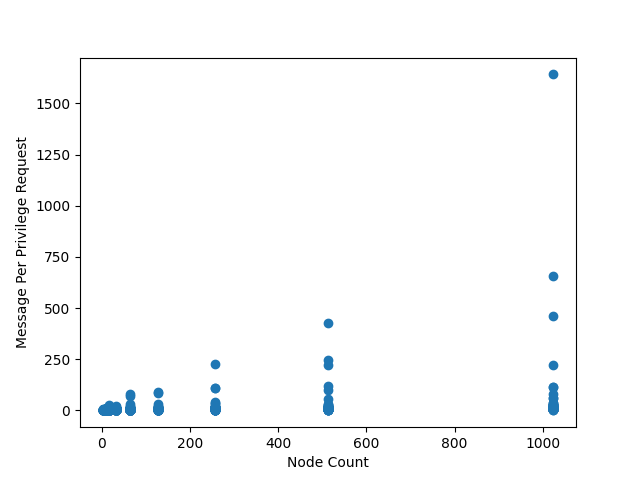
\includegraphics[scale=0.5]{figures/RaymondAlgorithmMessageComplexity.png}
    \caption{Raymond Algorithm Message Complexity}
    \label{fig:raymond_algoritm_message_complexity}
\end{figure}
\end{frame}

\subsection{Message Complexity - Node Count \& K}
\begin{frame}
\frametitle{Message Complexity - Node Count \& K}
\framesubtitle{}
\begin{figure}
    \centering
    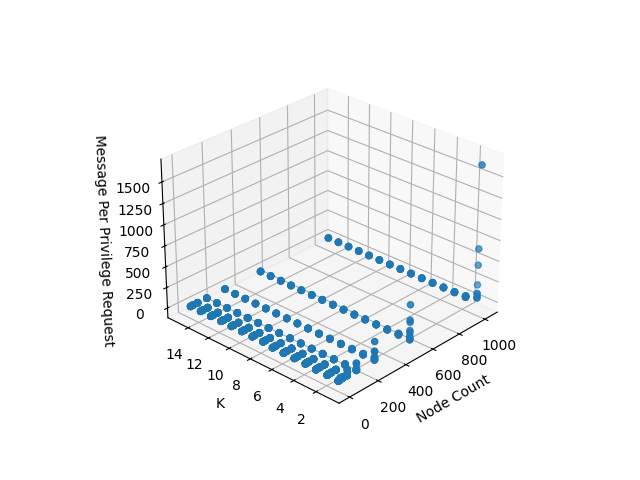
\includegraphics[scale=0.5]{figures/RaymondAlgorithmMessageComplexityPerK.png}
    \caption{Raymond Algorithm Message Complexity Per K}
    \label{fig:raymond_algoritm_message_complexity_per_k}
\end{figure}
\end{frame}

\section{Conclusions}
\begin{frame}
\frametitle{Conclusions}
\framesubtitle{}
\begin{itemize}
    \item Message Complexity
    \item Memory Complexity
    \item Node Failure
\end{itemize}

\end{frame}

\thankslide

\end{document}